\chapter{Information Gathering}

	The first phase in security assessment is focused on collecting as much information as 
	possible about a target application. Information Gathering is a necessary step of a penetration 
	test. This task can be carried out in many different ways. By using public tools (search engines),
	scanners, sending simple HTTP requests, or specially crafted requests, it is possible to force 
	the application to leak information, e.g., disclosing error messages or revealing the versions 
	and technologies used.

		\clearpage
		\section{OWASP-IG-001 - Spiders, Robots, and Crawlers}
			This phase of the Information Gathering process consists of browsing and capturing resources 
			related to the application being tested.  Web spiders/robots/crawlers retrieve a web page and 
			then recursively traverse hyperlinks to retrieve further web content.

			{\bf Black Box Testing} wget to retrieve information and Google Webmaster Tools to analyse 
			the retrived information from wget. Wget is a reqursive information retrival tool that collects 
			all information on the client side of an application. 

		\section{OWASP-IG-002 - Search Engine Discovery/ Reconnaissance}
			Search engines, such as Google, can be used to discover issues related to the web application
			structure or error pages produced by the application that have been publicly exposed.

			\begin{figure}[H]
				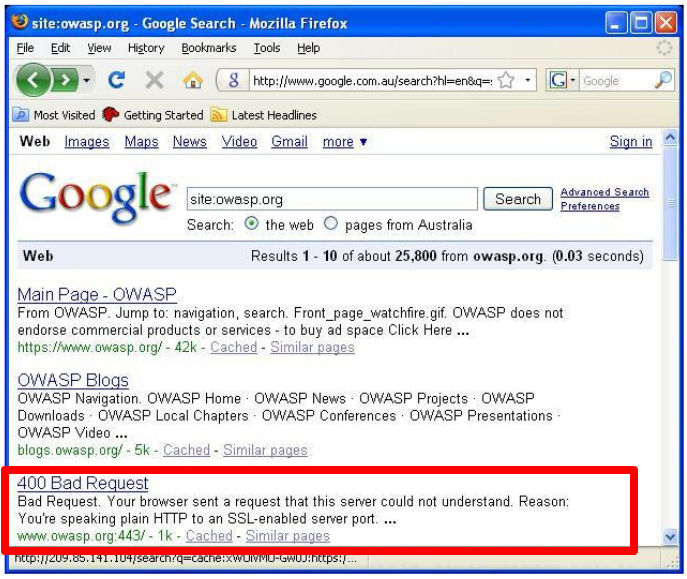
\includegraphics[width=\textwidth]{pics/searchEngine.png}
			\end{figure}



		\section{OWASP-IG-003 - Identify application entry points}
			Enumerating the application and its attack surface is a key precursor before any attack 
			should commence. This section will help you identify and map out every area within the 
			application that should be investigated once your enumeration and mapping phase has been 
			completed.

			Enumerating the application and its attack surface is a key precursor before any thorough 
			testing can be undertaken, as it allows the tester to identify likely areas of weakness. 
			This section aims to help identify and map out areas within the application that should be investigated once enumeration and mapping has been completed.

			Before any testing begins, always get a good understanding of the application and how the 
			user/browser communicates with it. As you walk through the application, pay special attention 
			to all HTTP requests (GET and POST Methods, also known as Verbs), as well as every parameter 
			and form field that are passed to the application. In addition, pay attention to when
			GET requests are used and when POST requests are used to pass parameters to the application. 
			It is very common that GET requests are used, but when sensitive information is passed, it 
			is often done within the body of a POST request. Note that to see the parameters sent in a 
			POST request, you will need to use a tool such as an intercepting proxy (for example,
			OWASP's WebScarab) or a browser plug-in. Within the POST request, also make special note of 
			any hidden form fields that are being passed to the application, as these usually contain 
			sensitive information, such as state information, quantity of items, the price of items, 
			that the developer never intended for you to see or change. This is typical data that an 
			attacker can tamper with. 

			Example:

			This example shows a POST request that would log you into an application.
			{\bf A simplified POST request:}
				\begin{itemize}
					\item {\bf POST} https://x.x.x.x/KevinNotSoGoodApp/authenticate.asp?service=login
					\item {\bf Host:} x.x.x.x
					\item {\bf Cookie:} 
   					SESSIONID = dGhpcyBpcyBhIGJhZCBhcHAgdGhhdCBzZXRzIHByZWRpY3RhYmxlIGNvb2tpZXMgYW5kIG1pbmUgaXMg
  					MTIzNA==
  					\item {\bf CustomCookie}=00my00trusted00ip00is00x.x.x.x00
  				\end{itemize}
			{\bf Body of the POST message:}
				\begin{itemize}
					\item user=admin\&pass=pass123\&debug=true\&fromtrustIP=true
				\end{itemize}



		\section{OWASP-IG-004 - Testing Web Application Fingerprint}
			Application fingerprint is the first step of the Information Gathering process; knowing 
			the version and type of a running web server allows testers to determine known 
			vulnerabilities and the appropriate exploits to use during testing.

			Web server fingerprinting is a critical task for the Penetration tester. Knowing the version 
			and type of a running web server allows testers to determine known vulnerabilities and the
			appropriate exploits to use during testing. There are several different vendors and versions 
			of web servers on the market today. Knowing the type of web server that you are testing
			significantly helps in the testing process, and will also change the course of the test. 
			This information can be derived by sending the web server specific commands and analyzing the 
			output, as each version of web server software may respond differently to these commands. 
			By knowing how each type of web server responds to specific commands and keeping this 
			information in a web server fingerprint database, a penetration tester can send these 
			commands to the web server, analyze the response, and compare it to the database of known signatures. 

			{\bf HTTP header field ordering:}
			The first method consists of observing the ordering of the several headers in the response. 
			Every web server has an inner ordering of the header. 

			{\bf Malformed requests test:}
			Another useful test to execute involves sending malformed requests or requests of nonexistent
			pages to the server.

			{\bf Automated Testing:}
			The tests to carry out in order to accurately fingerprint a web server can be many. 
			Luckily, there are tools that automate these tests. "httprint" is one of such tools. 
			httprint has a signature dictionary that allows one to recognize the type and the
			version of the web server in use. An example of on line tool that often delivers a lot 
			of information on target Web Server, is Netcraft. With this tool we canv
			retrieve information about operating system, web server used, Server Uptime, Netblock 
			Owner, history of change related to Web server and O.S.

		

		\section{OWASP-IG-005 - Application Discovery}
		Application discovery is an activity oriented to the identification of the web applications hosted on a web server/application
		server. This analysis is important because often there is not a direct link connecting the main application backend. Discovery
		analysis can be useful to reveal details such as web applications used for administrative purposes. In addition, it can reveal old versions of files or artifacts such as undeleted, obsolete scripts, crafted during the test/development phase or as the
		result of maintenance.

		\section{OWASP-IG-006 - Analysis of Error Codes}
		During a penetration test, web applications may divulge information that is not intended to be seen by an end user.
		Information such as error codes can inform the tester about technologies and products being used by the application.
		In many cases, error codes can be easily invoked without the need for specialist skills or tools, due to bad exception
		handling design and coding.
		Clearly, focusing only on the web application will not be an exhaustive test. It cannot be as comprehensive as the
		information possibly gathered by performing a broader infrastructure analysis.

